\documentclass[journal, a4paper]{IEEEtran}

\usepackage[left=2cm,right=1.5cm,top=1.5cm,bottom=1.5cm]{geometry}
\usepackage[backend=biber,sorting=ynt,style=alphabetic]{biblatex} 
\usepackage[caption=false, font=normalsize, labelfont=sf, textfont=sf]{subfig}
\usepackage{graphicx} 
\usepackage[utf8]{inputenc}
\usepackage[english]{babel}
\usepackage{csquotes}
\usepackage[parfill]{parskip}
\usepackage{url}    
\usepackage{hyperref}
\usepackage{authblk}
\usepackage{graphicx}
\usepackage{amsmath}
\usepackage{lipsum}

\addbibresource{references.bib} 

\graphicspath{{./images/}}

\hypersetup{
  colorlinks = true,
  linkcolor = blue,
  citecolor= blue,
  filecolor = blue,      
  urlcolor = blue,
  pdftitle = {Pedestrian Semaphore Classification - An Active Learning Approach}
  pdfauthor = {Miguel Rabuge, Gabriel Fernandes, Pedro Rodrigues},
  pdfsubject = {Pedestrian Semaphore Classification},
  pdfkeywords = {Artificial Intelligence, Machine Learning, Active Learning, 
  Autonomous Pedestrian Module, Image Classification},
  pdfproducer = {Latex with hyperref},
  pdfcreator = {pdflatex},
}

\begin{document}

\title{Pedestrian Semaphore Classification \\ An Active Learning Approach}
\author[1]{Gabriel Fernandes}
\author[2]{Miguel Rabuge}
\author[3]{Pedro Rodrigues}

\affil[1,2,3]{Department of Informatics Engineering, University of Coimbra, Portugal}{
  \makeatletter
  \renewcommand\AB@affilsepx{: \protect\Affilfont}
  \makeatother

  \makeatletter
  \renewcommand\AB@affilsepx{, \protect\Affilfont}
  \makeatother

  \affil[1]{gabrielf@student.dei.uc.pt}
  \affil[2]{rabuge@student.dei.uc.pt}
  \affil[3]{pedror@student.dei.uc.pt}
}

\maketitle

\thispagestyle{plain}
\pagestyle{plain}

\begin{abstract}

The environments, in which pedestrians with some form of disability circulate are 
often extremely risky, more so than for "healthy" pedestrians. Not only the 
environments are dynamic, and full of uncertainty but, since an impaired 
individual is not able to record quality sensory information his ability to 
navigate through the environment, without endangering himself, is compromised.
The most common solution for this problem is some form of personal companion, 
e.g “a guide dog”, that helps the individual circulate. Training these kinds of 
companions is often slow and expensive... We propose an “Active Learning” (AL) 
approach for training a classifier that could be integrated in an artificial 
personal companion module. In our work, we go on to compare our AL methodology
not only with state of the art models, but also with a model reported in recent paper 
on this topic. The obtained results show that models trained using this 
methodology can obtain the similar accuracies and with less data required.

\end{abstract}

\begin{IEEEkeywords}

Artificial Intelligence, Machine Learning, Active Learning, Autonomous Pedestrian Module, 
Image Classification.

\end{IEEEkeywords}

\section{Introduction}

Nowadays, there is a lot of effort being put into solving the problem of 
autonomous driving, not only because of research but also because of the security 
and comfort that autonomous vehicles may bring to our lives. Despite the fact of 
this problem being hard, it is made easy because of the environment
where the action of driving happens. There is a set of rules about how to drive, 
and where to drive to avoid potential accidents resulting in collisions with 
other vehicles, persons or objects. In other words, the environment is dynamic 
and risky, but it is less chaotic and more well-defined than others, which becomes 
more suited for the development of artificial intelligence approaches for training 
vehicles to be autonomous. 

To our knowledge, there has not been a lot of development of similar techniques 
for pedestrians, namely the ones that show some form of disability that could put 
them in danger if not accompanied by some form of personal companion. The 
pedestrian environment, unlike the one where vehicles circulate, does not have a 
set of rules describing the way people should walk nor a place where the action of 
walking takes place. The pedestrian may be forced to walk on a sidewalk, a 
(lighted) crosswalk, in rugged terrain or even in the car lane if no sidewalk 
exists. Additionally, the objects that a pedestrian needs to avoid obviously 
increases since a person needs not to worry only about walking itself, but also 
other obstacles with more unpredictable moving patterns. Therefore, the 
environment is often so chaotic that travelling by foot requires assistance and 
makes the problem less approachable from an artificial intelligence standpoint.

Since the problem of autonomous mobility for disabled pedestrians is not 
particularly developed, and the only way such mobility can be achieved is with 
the help of some form of companion, (like for instance a guide dog which requires 
a lot of training to successfully guide people), our contribution is to advance 
inside this field in terms of pedestrian semaphore detection and classification 
for a crosswalk-taking decision. The choice of an active learning (AL) approach 
is justified by the lack of datasets for this specific task. Therefore, AL is the 
perfect methodology to apply for this niche, but yet significant, application, 
since it can extract better accuracy from the models with fewer data.

In short, with this project we aim to explore an alternative methodology for 
this problem, by comparing the State-of-the-Art methods performance with our own, 
using various metrics. Our main objective is to build a classifier that should be 
fast to classify and highly accurate, without the need for large amounts of data.

We will base our research of a late breaking work entitled - "Flying Guide Dog: 
Walkable Drones and Transformer-based Semantic Segmentation" \cite{tan2021flying} 
- that uses a custom-made classification model based on a convolutional neural 
network (CNN) for semaphore detection on segmented images. Moreover, not only 
will we test our AL approach against this paper's CNN model, but we will build 
and train other State-of-the-Art CNN's in order to further study and justify 
the possibility of an AL approach to yield more efficient results.

\section{State Of The Art} \label{sota}

In the past few years, the State of the Art of image classifiers tends to revolve 
around Convolutional Neural Networks, due to the large amounts of data and
the processing power currently available, which have turned out to be highly 
rewarding when both conditions are true. Although the hardware available today
is really sophisticated and allows us to achieve good results through the use 
of CNN's for image recognition.

Regarding Active Learning, this approach aims to iteratively find the most 
informative data points to train the model, through the use of impurity measures. 
This methodology reveals being highly rewarding, generating good models with low 
data usage.

In the next sections we will discuss the state of the art convolutional neural
networks, focusing our analysis on the ``LeNet-5'' \cite{LeNet-5} and 
``AlexNet'' \cite{AlexNet} deep neural networks that we use later in work 
as a base for comparison and benchmark. We also refer the Active Learning 
methodology and point out some known strategies used with this method that 
we will also take advantage of in our experimental phase.

\subsection{Convolutional Neural Networks (CNN's)}

For the last years, deep learning has become a hot topic in the Artificial 
Intelligence landscape, with convolutional neural networks being one
of the most widely used methods for image classification, natural language
processing and computer vision tasks. Prior to this other methods were used
that relied on slow and time-consuming feature extraction methods, that 
with CNN's are not necessary since they are able to work with raw image data
without any need for feature pre-processing, therefore being perfect at picking up 
small patterns, which then are ``processed'' and combined through the multiple 
layers of the network, until the model can make sense of the provided data 
and classify what a given object really is.

Convolutional Neural Networks pose a great advantage in image classification, relying mainly on 
mathematical and algebraic models. In fact, many of the operations performed inside
the multiple layers of these deep networks often involve matrix multiplications
and other calculations that are highly vectorizable and parallelizable. 
The main drawbacks are that they are computationally demanding, often 
requiring graphical processing units (GPUs) for training more complex models 
and usually take some time to be trained to a level that make them efficient 
and accurate. In brief, by using CNN's the time and effort shifts from the 
user to the machine which somewhat advantageous, with the processing power
we have available to us nowadays.

The architecture of a CNN is mainly based on a multi-layer feed forward network
comprised of layers that learn from features processed by the layers before. 
The layers of these networks belong to one of these three types: convolutional, 
fully connected and pooling, existing many possible architectures made from 
arranging these in meaningful way.

\begin{figure}[htpb]
    \centering
    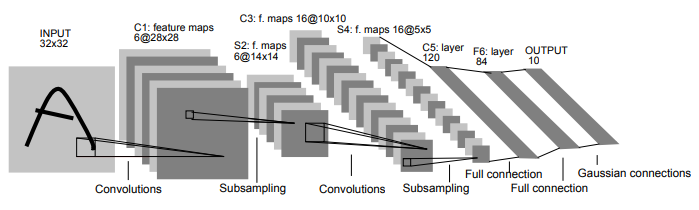
\includegraphics[scale=0.30]{LeNet-5}
    \caption[CNN]{Example architecture of a convolutional neural network 
      (LeNet-5); image from \parencite{LeNet-5}}
    \label{cnn}
\end{figure}

One well known attempt on CNN design was done by \textbf{Yann LeCun} with
the self-titled LeNet-5 \cite{LeNet-5}, which is known to have good performance in handwritten
digit recognition (MNIST) dataset and is still to this day considered a reference.
Overall this CNN consists on a five layer architecture that at a very high level 
is composed of two convolutional layers that serve as an encoder, and three 
fully connected layers that belong to the dense block of the network. 
A more recent attempt on a CNN design developed by \textbf{Alex Krizhevsky, Ilya Sutskever, 
and Geoffrey E. Hinton.}, the ``AlexNet'' \cite{AlexNet}. The CNN consists on an implementation 
on the LeNet-5 \cite{LeNet-5} but much deeper, having a total number of layers that amount to 
eight. Architecturally, the first five layers consist of convolutional layers (oftentimes 
appearing interleaved with pooling layers) and the last three are fully connected layers.

These CNN designs have proven to have good performance and have been considered state of the art
although other designs may be more effective for different datasets. For instance, on the
``Pedestrian and Vehicle Traffic Lights'' (PVTL) dataset \cite{PVTL} the authors used their own
implementation of a simple CNN (5 convolutional layers + 3 fully connected layers), claiming that 
it was able to achieve 83\% accuracy; furthermore, by using  a fine tuned CNN based on the 
``ResNet'', another state of the art CNN provided in the \textit{keras} python library, they 
were able to obtain accuracies of 90\%, both over a 25 epochs training.

Overall the results obtained by using state of the art CNN based models for image 
classification are promising and, when properly tuned, tend to be even better suited for 
each specific need. Our aim, with our work, is to further explore other possibilities for 
improving these models through the use of other techniques, such as active learning.

\subsection{Active Learning}

On active learning \textbf{Burr Settles} \cite{settles.tr09, pmlr-v16-settles11a} describes
it as being a method for further improving the performance of machine learning models, making
them achieve greater accuracies. In this semi-supervised learning method, through the usage of 
queries of unlabeled data made to an \textit{oracle}, the active learner is not only able to 
choose the data from which it learns but also choose the data where the model is most 
uncertain about and learn from it, therefore increasing the learning process speed.

The active learning cycle is a sequence of steps by which an active learner attempts 
to iteratively improve the performance of the model. One of the most common active leaning 
cycle methodologies is the pool-based sampling active learning, in which the queries made to 
the \textit{oracle} select examples from a ``pool'' of  unlabeled instances in accordance 
to a given strategy that should take into account the information gain that a given instance 
may add to the model.

\begin{figure}[htpb]
    \centering
    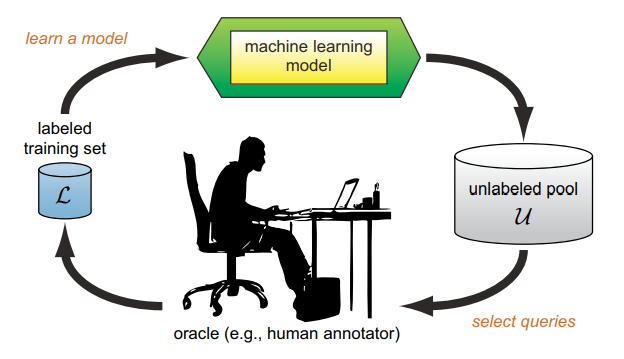
\includegraphics[scale=0.38]{AL}
    \caption[AL]{A pool-based active learning cycle; image from \parencite{settles.tr09}}
    \label{al}
\end{figure}

There exists a wide variety of query strategies, namely: query-by-committee, expected model change,
expected error reduction, uncertainty sampling, etc... .One of the most commonly used query 
strategies, and that we will use in the experimental phase of our work is 
\textit{uncertainty sampling} and consists in a framework where the queries to the model, made by 
the active learner, are done in such a way as to select the instances from the pool which the 
learner is \textit{less confident} about (\ref{eq:1}). The standard measure of uncertainty used 
by this method consists in the choice of the instance whose prediction conveys the 
lowest confidence. Other measures often considered are the \textit{entropy} (\ref{eq:2}) 
and the probability difference between the two most likely labels (\ref{eq:3}); these 
strategies correspond to the so called \textit{entropy sampling} and \textit{margin sampling}
strategies respectively.

\begin{equation}
    \label{eq:1}
    \large{x^*_{LC} = \operatorname*{argmax}_x 1 
                       - P_{\theta}(\hat{y}_{1}|x)}
\end{equation}

\begin{equation}
    \label{eq:2}
    \large{x^*_{H} = \operatorname*{argmax}_x 
                   \sum_{i}{P_{\theta}(y_{i}|x) 
                   \cdot 
                   \log{P_{\theta}(y_{i}|x)}}}
\end{equation}

\begin{equation}
    \label{eq:3}
    \large{x^*_{M} = \operatorname*{argmin}_x 
                    P_{\theta}(\hat{y}_{1}|x) 
                    - P_{\theta}(\hat{y}_{2}|x)}
\end{equation}

Above are shown in mathematical notation the possible metrics for picking an instance under the 
\textit{uncertainty sampling} active learning framework. In the formulas above, $\theta$ represents 
the model and $x$, $y$ instance labels. For formulas (\ref{eq:1}, \ref{eq:3}),
$\hat{y}_{k}=\operatorname*{argmax}_y P_{\theta}(y|x)$ denotes the $k$-th most probable 
instance label under the model $\theta$. \cite{settles.tr09}.

Having discussed the state of the art active learning methodologies we will now move on to the
experimental phase of our work where we will put these methods in practice and check if we can 
extract any benefits of their usage.

\section{Materials: Datasets and Frameworks}

In terms of pedestrian assistive agents, there has not been a lot of research 
related to it since a ``Pedestrian Assistant'' is a relatively recent topic. 
The most recent scientific paper that we found for it, uses a standard 
state of the art CNN for the pedestrian traffic lights detection and 
classification module of their project, trained by using a newly introduced 
dataset “Pedestrian and Vehicle Traffic Lights” (PVTL), \cite{PVTL} which is a 
preprocessed subset of \href{https://www.mapillary.com/}{Mapillary’s} vast image data 
set that we are going to make use throughout our work.

\begin{figure}[htpb]
    \centering
    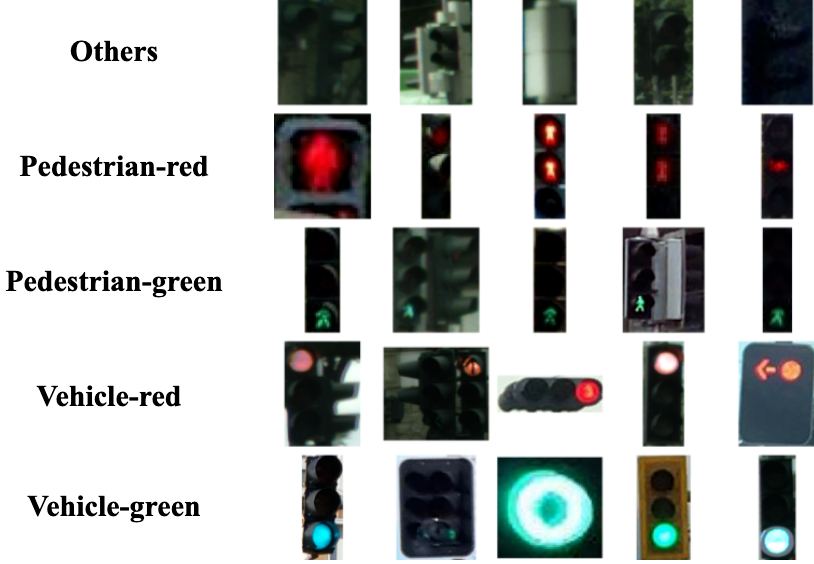
\includegraphics[scale=0.28]{PVTL-Preview}
    \caption[PVTLD]{Pedestrian Vehicle and Traffic Lights dataset sample; 
                    image from \parencite{PVTL}}
    \label{pvtld}
\end{figure}

This dataset is composed by a series of images of semaphores of different types, colors 
and shapes. The data in this dataset is grouped into five different classes:
``Others'', ``Pedestrian-green'', ''Pedestrian-red'', ``Vehicle-red'', ``Vehicle-green''.
The image above (figure \ref{pvtld}) illustrates the different dataset classes and shows 
some samples of images that may be found in each class. Each one of these classes contains about 
300 images that we preprocessed in order to standardize the input. The image preprocessing step 
will be discussed in the ``Dataset Preprocessing'' section \ref{dpp}.

The whole project was developed using the python programming language and making use 
of multiple python frameworks that provided us with tools for image processing, deep neural network
model construction/training and active learning. A list of frameworks used in our work can 
be consulted in the ``Frameworks'' section \ref{frmw}.

For consistency and reproducibility purposes all experiments were made in a single machine 
whose specifications are shown in the table below.

% TODO: Maybe complete with more detailed specs?
\begin{table}[h]
    \label{tab:1}
    \caption{Benchmark Machine specifications.}
    \centering
    \scalebox{1.25}{ 
        \begin{tabular}{|l|l|}
            \hline
            CPU & AMD Ryzen™ 7 1700 Processor 3.0GHz \\ \hline
            RAM & 16GB DDR4                          \\ \hline
            GPU & Nvidia GeForce 1070                \\ \hline
        \end{tabular}
    }
\end{table}

\subsection{Dataset Preprocessing} \label{dpp}

In order to make the images from the \cite{PVTL} dataset ready to be used the models 
developed, we needed to address the fact that all the images had different dimensions.
This fact made it unfeasible to feed the images as is directly to a CNN and 
required us to reshape all the images in dataset. After a careful look 
at the dataset, we decided that we would work with images with dimensions 224x224 pixels and
proceeded to proportionally re-scale all the images to said dimensions. In the case of the images
which a re-scaling event would result in the image being shrunk down, the regions left empty 
were filled with a black strip, therefore minimizing any interference in the model's predictions.

\subsection{Frameworks} \label{frmw}

In terms of frameworks, in this project besides all the standard python libraries, we used
the following frameworks:

\begin{itemize}
    \item \textbf{Pillow} \cite{PIL}: For loading the dataset images.
    \item \textbf{TensorFlow} \cite{tensorflow}: For CNN model construction.
    \item \textbf{modAL} \cite{modAL}: For the AL cycle implementation.
    \item \textbf{openCV} \cite{openCV}: For image preprocessing (e.g re-scalling/padding).
\end{itemize}

\section{Experimental Setup}

In this section we present the experimental setup for studying the effectiveness/performance of 
and active learning approach on pedestrian semaphore classification. In the first sub-section 
\ref{impl} we discuss the implementation made in the scope of this project and in the second 
\ref{exp} we move on to talk about the design of the experiments / experimental scenario.

\subsection{Implementation} \label{impl}

% TODO: check the writing on this section please!

For the purposes of work and in order to implement the active learning cycle we needed
well designed models that would allow us to observe the active learning contribution.

First of all, we started by implementing some state of the art CNN's since these are
well known models and have proved to yield a good performance in image classification,
therefore serving as the control group of our experiments. That being said, 
the state of the art CNN's we ended up choosing for implementation were 
LeNet \cite{LeNet-5} and the AlexNet \cite{AlexNet} whereas both are similar but 
architecturally one CNN has more depth than the other.

Afterwards, in order to later establish further comparison with the most recent 
work (to our knowledge) on personal companions for impaired pedestrians \cite{tan2021flying},
we decided to implement one of the CNN's used in said work. With this, our main goal was not 
only compare the performance with state of the art CNN's (control group), but also later 
check if the AL approach would better the performance obtained by this CNN that was 
custom built for this particular problem. The architecture of the CNN as previously 
discussed in the state of the art section (\ref{sota}), that at a very high level, 
is comprised of 5 convolutional layers followed by 3 fully connected layers. 
Throughout our work we will refer back to this CNN as \textit{FlyNet}.

After the models were implemented it was time to introduce the active learning cycle
into the models. For this work we decided to use uncertainty based sampling, implementing
the multiple sampling strategies in order to assess which one was the best fit for our goals. 

\subsection{Experimental Scenario} \label{exp}

Having the dataset loaded and all the necessary components of the AI system implemented we
proceeded to testing it. The experiences conducted were designed to test the multiple models
implemented as well as how they behaved when the active learning loop was introduced. Be that
as it may, we ran each CNN model with 30 different seeds (from seed with number 0 to 29) with a
training duration of 25 epochs, hence obtaining representative results of the performance of the
CNN and avoiding a potential bias that running with the same seed might have introduced. The choice
for 25 epochs training duration was due to the accuracy stabilization observed after 15 epochs,
also in the \cite{tan2021flying} paper they used the same parametrization which inclined towards us 
using this value.

\begin{figure}[htpb]
    \centering
    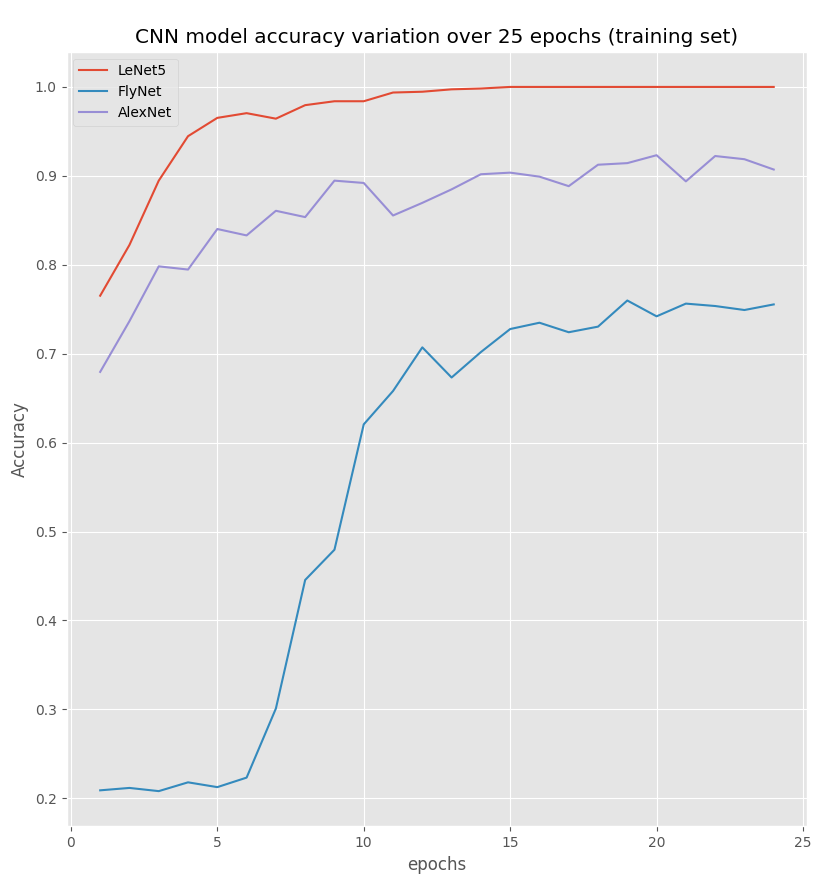
\includegraphics[scale=0.4]{CNNAccuracy}
    \caption[CNNAcc]{Accuracy evolution over 25 epochs for the multiple CNN's; 
        training set results; seed 42.}
    \label{CNNAcc}
\end{figure}

Afterwards, we tested the active learning loop on each of the trained models using the
multiple query strategies implemented (\ref{impl}). As the parametrization of the the AL loop,
we used an initial size of the training data of 600 known labels, a query size of 60 labels and, 
as the maximum number of queries made in the active learning loop, 11 queries, having concluded 
a total of 8 queries per learning strategy until the pool of unlabeled data was depleted. 
Furthermore, after each query, the model was re-trained with 25 epochs in order to 
be able to learn the new examples provided. Last but not least, on the experiments made the 
considered metric was the accuracy obtained by the model using AL when compared
with the model without it. Our main interest is to observe the impact in terms of performance
(accuracy) and its evolution, e.g number of queries needed to obtain results the match the original model
without the AL cycle.

\section{Results}

We started by looking at the performance of the models when considering the raw models without
the active cycle implemented into it. The results obtained can be observed in the following table:

\begin{table}[htpb]
    \centering
    \caption{Average CNN's accuracy over 30 runs (test set)}
    \scalebox{1.25}{ 
        \begin{tabular}{|c|c|}
            \hline
            CNN                       & Accuracy        \\ \hline
            LeNet5                    & 0.809           \\ \hline
            AlexNet                   & 0.868           \\ \hline
            FlyNet                    & 0.417           \\ \hline
        \end{tabular}
    }
    \label{tab:2}
\end{table}

The results (table \ref{tab:2}) show that both LeNet5 and AlexNet show good performances on 
the testing set, unfortunately the FlyNet network implementation performs poorly, which 
is something unfortunate taking into account the accuracy reported by the authors of the 
CNN \cite{tan2021flying} on their tests. These results on the FlyNet may be 
implementation dependent but the original authors do not provide any details about that so 
we can reproduce their work, leaving us to establish our analysis
strictly with our implementation which yields this performance. Nonetheless, the results may 
still be used to assess the quality of the AL methodology we wish to test.

In the following graphics we show the comparison between the performances obtained when 
comparing the results obtained from running, on the test set, the raw CNN's against the 
results obtained when the AL cycle (with multiple query strategies) was introduced 
(figure \ref{ALP1}). We also show the results obtained when comparing the performances 
obtained by the CNN's with AL, in the training set against the ones obtained in the testing set (figure \ref{ALP2}).

\begin{figure*}[htpb] 
    \centering
    \subfloat[LeNet5\label{1a}]{
       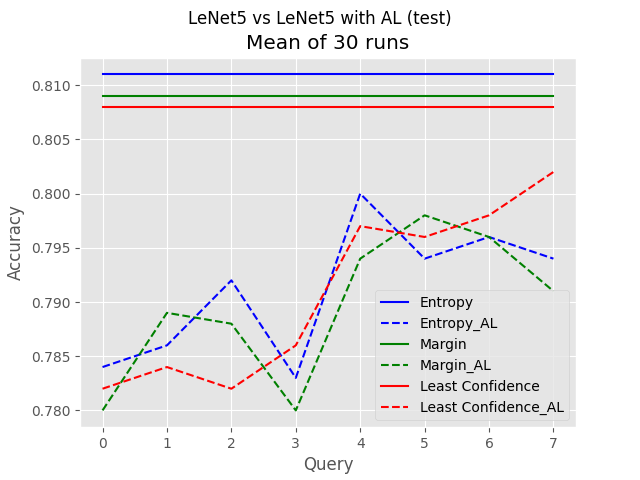
\includegraphics[scale=0.4]{LeNet5_VS_AL.png}
    }
    \hfill
    \subfloat[AlexNet\label{1b}]{
        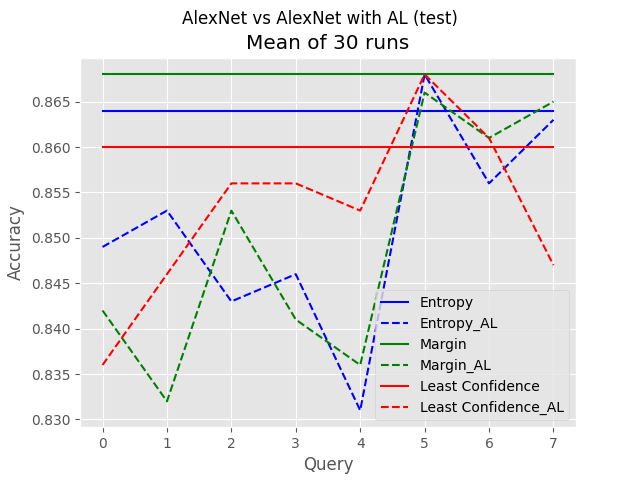
\includegraphics[scale=0.4]{AlexNet_VS_AL.png}
    }
    \hfill
    \subfloat[FlyNet\label{1c}]{
        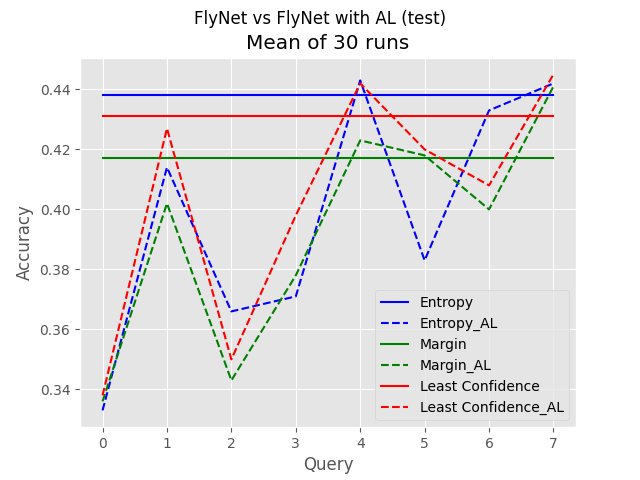
\includegraphics[scale=0.4]{FlyNet_VS_AL.png}
    }
    \caption{Performance evolution for the CNN's: LeNet5 (figure \ref{1a}), AlexNet (figure
    \ref{1b}), FlyNet (figure \ref{1c}), compared with CNN's + AL with different query 
    strategies (entropy sampling (blue), margin sampling (green), least confidence (red) sampling).}
    \label{ALP1} 
\end{figure*}

\begin{figure*}[htpb]
    \centering
    \subfloat[LeNet5\label{2a}]{
       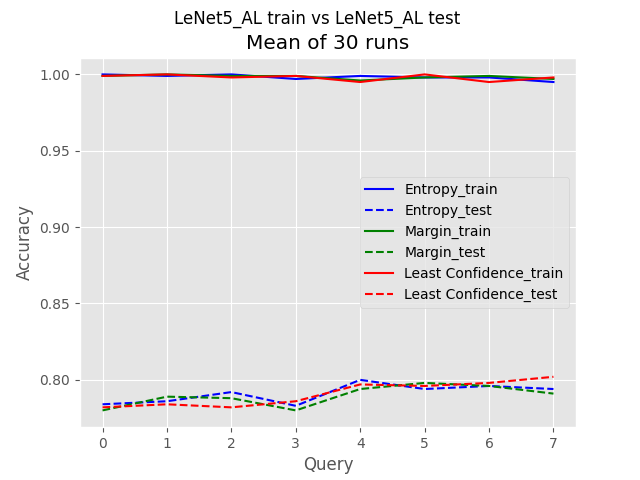
\includegraphics[scale=0.4]{LeNet5_TT_AL.png}
    }
    \hfill
    \subfloat[AlexNet\label{2b}]{
        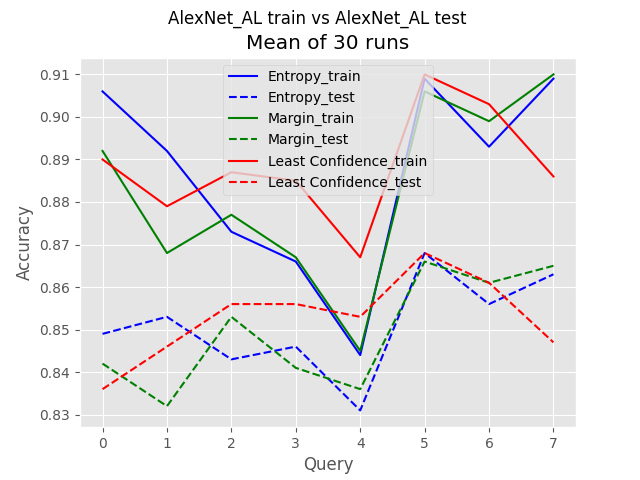
\includegraphics[scale=0.4]{AlexNet_TT_AL.png}
    }
    \hfill
    \subfloat[FlyNet\label{2c}]{
        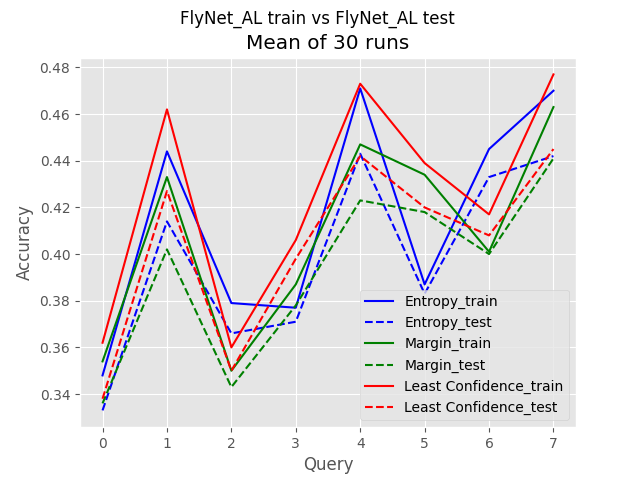
\includegraphics[scale=0.4]{FlyNet_TT_AL.png}
    }
    \caption{Performance evolution and differences between training and testing sets for the 
    CNN's + AL: LeNet5 (figure \ref{2a}), AlexNet (figure \ref{2b}), FlyNet (figure \ref{2c}), 
    with different query strategies (entropy sampling (blue), 
    margin sampling (green), least confidence (red) sampling)}
    \label{ALP2} 
\end{figure*}

\section{Discussion and Conclusions}

As we can observe from the results we obtained, in general the accuracies we got from using
the CNN's with AL are very close to the ones obtained when using the raw CNN's with no AL,
using a smaller amount of instances. This is visible on the multiple plots on figure \ref{ALP1}. 

When comparing the performance difference
between the training set and the testing sets, figure \ref{ALP2}, we can see that the results 
obtained are worse when we look at the test set in comparison to the training set. This is
to be expected since the testing set contains data that the model has never seen,
which leads it to have less accuracy. Nonetheless, the accuracy difference between training/test
sets for the AlexNet and FlyNet CNN's is not blatant, showing that these models have great 
generalization capabilities, therefore being able to classify new samples accurately.
In the case of the LeNet5, the results show that this CNN's is most certainly overfiting on 
the training data. This is evident since, with the training set the model is able to obtain
accuracies that round 1.0, but when it is exposed to the test set it is only able to reach
accuracies of about 0.80.

In conclusion, we are confident that the results obtained are representative of the improvements
that an AL approach for training classifiers may bring, in the sense that we can train the
models with less data. When comparing to state of the art methods, and the model in the \cite{tan2021flying} paper, results also show that this methodology is really competitive.

\section{Future Work}

From our research, we realized that there is still a lot to be done in this field.
In fact, the development of assistive systems for impaired pedestrians is a fairly 
recent topic from the point of view of AI research, much so that with our work, we only 
touched a small topic which is the improvement of semaphore classification techniques 
for these systems by using active learning techniques. We feel that two main things must 
be done in the near future in order to enable more research in this area. First of all 
the creation of more datasets containing a wider variety of obstacles that a pedestrian may 
encounter is of paramount importance. The existence of more datasets will allow the 
same methodology discussed in this work to be used in the classification of more objects, 
therefore allowing for the development of a more capable and complete assistive systems. 
Last but not least, regarding our work in particular, the experimentation with other active 
learning query strategies is an important topic that we leave as future work, as other 
methodologies may be able to achieve even better results. 

\printbibliography

\end{document}
